% !TEX program = lualatex
% Generated by new_homework.sh — Math 104 Homework 5
\documentclass[11pt]{article}

\usepackage{fontspec}
\usepackage{microtype}
\usepackage{mathtools,amssymb,amsfonts,amsthm,bm}
\usepackage{enumitem}
\usepackage{booktabs,array,xcolor}
\usepackage{geometry,fancyhdr,setspace}
\usepackage{pdfpages}
\usepackage[hidelinks]{hyperref}
\usepackage[nameinlink,noabbrev]{cleveref}

% ---------- Page and paragraph rhythm (matches lecture/solutions templates) ----------
\geometry{margin=1in,headheight=15pt}
\setstretch{1.12}
\setlength{\parindent}{0pt}
\setlength{\parskip}{0.55em plus 0.12em minus 0.08em}
\setlength{\abovedisplayskip}{0.8em plus 0.2em minus 0.1em}
\setlength{\belowdisplayskip}{0.8em plus 0.2em minus 0.1em}
\allowdisplaybreaks[3]
\setlist{leftmargin=*,topsep=0.35em,itemsep=0.15em,parsep=0pt}

% ---------- Metadata ----------
\newcommand{\studentname}{Keshav Ramamurthy}
\newcommand{\coursename}{Math 104}
\newcommand{\courselongname}{Real Analysis}
\newcommand{\assignment}{Homework 5}
\newcommand{\term}{Fall 2026}

% ---------- Core notation (same as ~/.config/nvim/textemplate.tex) ----------
\newcommand{\N}{\mathbb{N}}
\newcommand{\Z}{\mathbb{Z}}
\newcommand{\Q}{\mathbb{Q}}
\newcommand{\R}{\mathbb{R}}
\newcommand{\C}{\mathbb{C}}
\newcommand{\F}{\mathbb{F}}
\newcommand{\K}{\mathbb{K}}
\newcommand{\E}{\mathbb{E}}
\newcommand{\Prob}{\mathbb{P}}
\newcommand{\1}{\mathbf{1}}
\newcommand{\eps}{\varepsilon}
\newcommand{\dd}{\,\mathrm{d}}
\newcommand{\abs}[1]{\left\lvert#1\right\rvert}
\newcommand{\norm}[1]{\left\lVert#1\right\rVert}
\newcommand{\ip}[2]{\left\langle#1,#2\right\rangle}
\newcommand{\set}[1]{\left\{#1\right\}}
\newcommand{\ceil}[1]{\left\lceil#1\right\rceil}
\newcommand{\floor}[1]{\left\lfloor#1\right\rfloor}
\newcommand{\given}{\,\middle\vert\,}
\newcommand{\indep}{\perp\!\!\!\perp}
\newcommand{\wh}[1]{\widehat{#1}}
\newcommand{\deriv}[2]{\frac{\mathrm{d}#1}{\mathrm{d}#2}}
\newcommand{\pderiv}[2]{\frac{\partial#1}{\partial#2}}
\newcommand{\lto}{\longrightarrow}
\newcommand{\st}{\text{ such that }}
\DeclareMathOperator{\Aut}{Aut}
\DeclareMathOperator{\End}{End}
\DeclareMathOperator{\Gal}{Gal}
\DeclareMathOperator{\Hom}{Hom}
\DeclareMathOperator{\Ker}{ker}
\DeclareMathOperator{\im}{im}
\DeclareMathOperator{\rank}{rank}
\DeclareMathOperator{\nullity}{nullity}
\DeclareMathOperator{\Span}{span}
\DeclareMathOperator{\tr}{tr}
\DeclareMathOperator{\diag}{diag}
\DeclareMathOperator{\spec}{spec}
\DeclareMathOperator{\ord}{ord}
\DeclareMathOperator{\supp}{supp}
\DeclareMathOperator{\diam}{diam}
\DeclareMathOperator{\Var}{Var}
\DeclareMathOperator{\Cov}{Cov}
\DeclareMathOperator*{\argmin}{arg\,min}
\DeclareMathOperator*{\argmax}{arg\,max}

% ---------- Statement environments ----------
\newtheorem{problem}{Problem}
\newtheorem{theorem}{Theorem}
\newtheorem{lemma}{Lemma}
\newtheorem{proposition}{Proposition}
\newtheorem{corollary}{Corollary}
\theoremstyle{definition}
\newtheorem{definition}{Definition}
\newtheorem{example}{Example}
\newtheorem{remark}{Remark}

% ---------- Solution machinery (matches solutions.tex / textemplate.tex) ----------
\newenvironment{solution}{\begin{proof}[Solution]}{\end{proof}}
\newenvironment{answer}{\begin{proof}[Answer]}{\end{proof}}
\renewcommand{\qedsymbol}{\(\square\)}
\newcommand{\exercise}[1]{%
  \par\goodbreak\medskip\noindent\textbf{Exercise #1}\par\nopagebreak\smallskip\nopagebreak}
\newcommand{\exref}[1]{\textsf{\textbf{Exercise~#1}}}
\newenvironment{claim}{\par\smallskip\noindent\textit{Claim.}\ }{\par\smallskip}
\newenvironment{idea}{\par\smallskip\noindent\textit{Idea.}\ }{\par\smallskip}
\newenvironment{proofsketch}{\par\smallskip\noindent\textit{Proof sketch.}\ }{\par\smallskip}

% ---------- Header ----------
\pagestyle{fancy}
\fancyhf{}
\fancyhead[L]{\coursename}
\fancyhead[C]{\assignment\ — my solutions}
\fancyhead[R]{\studentname}
\fancyfoot[C]{\thepage}

\begin{document}

% ---------- Title ----------
\begin{center}
  {\Large\sffamily\bfseries \coursename\ -- \courselongname}\par\vspace{3pt}
  {\sffamily \assignment\ — my solutions}\par\vspace{3pt}
  {\small\sffamily \term\quad\textbullet\quad \studentname}
\end{center}
\medskip
\hrule
\bigskip

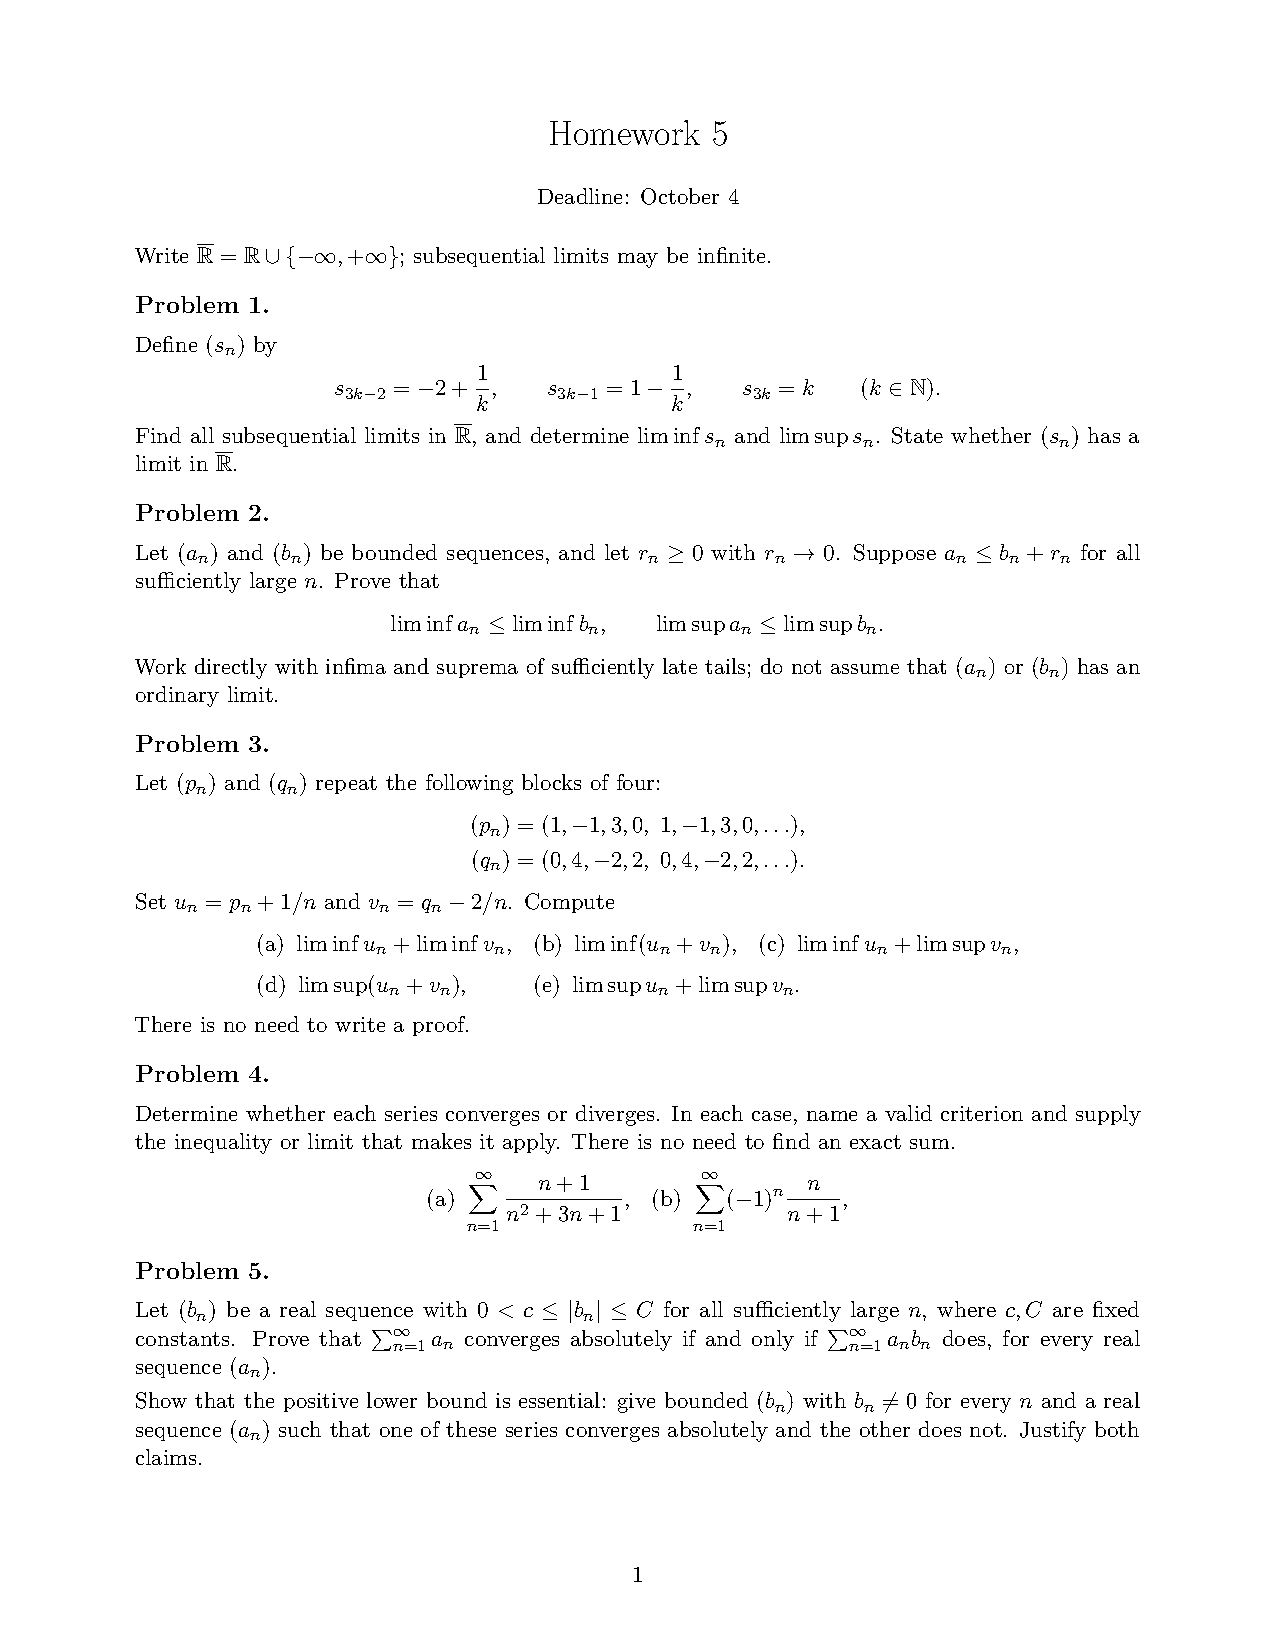
\includepdf[pages=-,pagecommand={\thispagestyle{empty}}]{HW5.pdf}
\clearpage

\section*{Solutions}
\subsubsection*{Problem 1}
\begin{solution}
The terms split into three subsequences:
\[
s_{3k-2}\longrightarrow -2,\qquad
s_{3k-1}\longrightarrow 1,\qquad
s_{3k}\longrightarrow +\infty.
\]
These are all the subsequential limits. Therefore,
\[
\liminf_{n\to\infty}s_n=-2,\qquad
\limsup_{n\to\infty}s_n=+\infty.
\]
The subsequences tending to $-2$ and $1$ have different limits, so
$(s_n)$ does not have a limit in $\mathbb{R}$.
\end{solution}
\subsubsection*{Problem 2}
\begin{solution}
For $N$ large enough, $a_n\leq b_n+r_n$ holds for every $n\geq N$. Set
\[
R_N=\sup_{n\geq N}r_n.
\]
Since $r_n\to0$ and $r_n\geq0$, we have $R_N\to0$. For every $n\geq N$,
$a_n\leq b_n+R_N$. Taking the infimum and supremum over this same tail gives
\[
\inf_{n\geq N}a_n\leq \inf_{n\geq N}b_n+R_N,\qquad
\sup_{n\geq N}a_n\leq \sup_{n\geq N}b_n+R_N.
\]
As $N\to\infty$, the tail infima and suprema approach the corresponding
lim infs and lim sups, while $R_N\to0$. Thus
\[
\liminf_{n\to\infty}a_n\leq\liminf_{n\to\infty}b_n,\qquad
\limsup_{n\to\infty}a_n\leq\limsup_{n\to\infty}b_n.
\]
\end{solution}
\subsubsection*{Problem 3}
\begin{solution}
The terms $1/n$ and $2/n$ tend to zero, so the repeating blocks determine
the lim infs and lim sups. For $u_n+v_n$, the block is $(1,3,1,2)$.
Therefore,
\[
\begin{aligned}
\text{(a)}\;&\liminf u_n+\liminf v_n=-1+(-2)=-3,\\
\text{(b)}\;&\liminf(u_n+v_n)=1,\\
\text{(c)}\;&\liminf u_n+\limsup v_n=-1+4=3,\\
\text{(d)}\;&\limsup(u_n+v_n)=3,\\
\text{(e)}\;&\limsup u_n+\limsup v_n=3+4=7.
\end{aligned}
\]
\end{solution}
\subsubsection*{Problem 4}
\begin{solution}
For (a), the terms are positive and
\[
\frac{n+1}{n^2+3n+1}>\frac{1}{n+3},
\]
since $(n+1)(n+3)>n^2+3n+1$. The series $\sum_{n=1}^\infty 1/(n+3)$
is a shifted harmonic series and diverges, so the comparison test shows
that the given series diverges.

\par For (b), the terms do not tend to zero:
\[
\left|(-1)^n\frac{n}{n+1}\right|=\frac{n}{n+1}\longrightarrow 1.
\]
By the nth-term test, this series diverges.
\end{solution}
\subsubsection*{Problem 5}
\begin{solution}
    We will first show the direction that $\sum_{i=1}^{n} a_i$ converges implies
    $\sum_{i=1}^{n} a_ib_i$ converges given that $$0 < c < |b_n| \le C$$ for all sufficiently
    large  n.
\par    Then, notice that (for sufficiently large n)
    $$\sum_{i = 1}^{n}a_i \le \sum a_i C \le C \sum a_i$$ and similarly:
        $$c\sum a_i \le \sum a_i b_i \le C\sum a_i$$
    Both $c\sum
    a_i$  and $C \sum a_i$ converge, then $\sum a_ib_i$ is bounded and must converge. 
    To show the converse, we start from $\sum a_i b_i$ converging, and we wish to prove
    that this implies $\sum a_i$ must converge.
    In order to do so, we again bound it like the previous step, noticing for
    sufficiently large $n$ that 
    $$\sum a_i c \le \sum a_i b_i \le a_iC$$
        where $c, C>0$

% Write your proof, calculation, or argument here.
\end{solution}

\end{document}
